\documentclass[]{elsarticle}
\usepackage{amsmath}

\begin{document}

\section{Abstract}

\section{Introduction} \label{sec:introduction}
Polar Mesospheric Clouds (PMCs), found at altitudes near or beyond 80 km, are composed of ice particles that condense out of their cold environs. They are most prevalent at or around the summer (winter) solstice in the Northern (Southern) hemisphere when temperatures are lowest. Ground-based observers refer to PMCs as Noctilucent Clouds (NLCs), due to their quality of shining most brightly at evening or morning twilight. PMCs are being tracked more closely in recent years by a number of missions due to their suspected correlation with rising global temperatures and CO$_{2}$ and H$_{2}$O concentrations \cite{Lubken2018}. As the greenhouse effect takes hold, adiabatic cooling takes place in the mesosphere, resulting from global meridional circulation \cite{Suzuki2013}. Such a phenomenon, itself driven by gravity wave acceleration, provides the required temperatures for H$_{2}$O condensation. The nucleation source is thought to be meteoric smoke particles residing in the stratosphere and mesosphere resulting from ablation \cite{Hervig2012}. The physical properties of PMCs, such as particle size, shape and density, can be used to inform upon surrounding atmospheric conditions and dynamics. Although it is firmly held that ice particles comprise the clouds, it is often left to microphysical models to explain the observed size distributions \cite{Cossart1999} \cite{Bailey2015} and absorption properties. In particular, the particle shape, while known to be non-spherical \cite{Eremenko2005}, is a lot more ambiguous \cite{Rapp2007} and often relies on a priori assumptions. 
As a result of this interest, PMCs have been studied through ground, rocket and space observations with increasing sophistication and intent. Most recently, NASA's AIM/SOFIE (Aeronomy of Ice in the Mesosphere/Solar Occultation For Ice Experiment) and AIM/CIPS (Cloud Imaging and Particle Size) instruments have been able to produce key PMC characteristics. Before that, the Michelson Interferometer for Passive Atmospheric Sounding (MIPAS) on board the Envisat satellite was able to derive ice volume densities, at all times of day, from infrared emission signatures. From the ground, lidar measurements, from both the Southern \cite{Chu2013} and Northern \cite{Baumgarten2010} Hemispheres, have been used to detect larger ($\approx$20 nm) PMC particles and their respective size distributions.
In their paper, Eremenko et al. \citey{Eremenko2005} did a select analysis on spectral observations from the Atmospheric Chemsity Experiment Fourier Transform Spectrometer (ACE-FTS) deemed to have been indicative of a PMC. They examined $\approx$30 spectra from 2004 at polar latitudes and tangent altitudes between 75 and 85 km. One of the primary conclusions was that these clouds predominantly contained nonspherical ice crystals in the size range 59 $\pm$ 5 nm. 
Here, we will present the results of a full census on all spectra from the ACE mission start in August 2003 to today. Upon first deciding the presence or absence of a cloud, the spectra will be fit so as to glean as much information as possible about them. Section \ref{sec:instrument} will begin by fully describing the ACE-FTS on board Scisat-1 and the advantages that it offers versus other missions in its ability to detect and analyse PMCs. Section \ref{sec:methods} will explain the methods by which detections were identified and how the T-matrix algorithms of Mishchenko and Travis \cite{Mishchenko1998} were used to fit the spectra. Our results will be shown in Section \ref{sec:results}, while a comparison with other missions will be undertaken in Section \ref{sec:disc}. Finally, Section \ref{sec:conc} will issue conclusions and offer suggestions for ways forward.
\underline{}
\section{ACE-FTS} \label{sec:instrument}
The Atmospheric Chemistry Experiment (ACE) \cite{Bernath2017} \cite{Bernath2005}, launched in 2003, and its on-board infrared Fourier transform spectrometer (FTS), makes high-resolution (0.02 cm$^{-1}$) spectral measurements in solar occultation mode. The foremost goal of ACE was to achieve a thorough understanding of the chemistry underpinning the evolution of ozone in the stratosphere and upper troposphere, especially around the Arctic. Today, the ACE Science Operations Centre (SOC) processes more than 60 atmospheric constituents, an achievement that has led to many varied scientific discoveries. Along with the FTS, ACE also has a two-channel imaging camera \cite{Gilbert2007} initially designed to detect obscuring clouds. However, its sensitivity is such that PMCs cannot usually be seen. ACE traverses a low-Earth, high-inclination orbit, allowing it to probe all latitudes from the tropics to the poles. At this orientation, the orbit is repetitive on a yearly basis, meaning that coverage zones can be co-added to increase the sample size. 

\section{Methods} \label{sec:methods}
In spite of the bias of PMCs toward certain latitudes, altitudes and times of year, the entire ACE data set was searched for possible signatures. We registered a detection upon identification of the 3200 cm$^{-1}$ O-H stretch band vibrational mode, in a manner similar to Petelina and Zasetsky \cite{Petelina2009} \cite{Petelina2011}. The chosen threshold relative to the background level was $0.99$ in transmission. From February 2004 - April 2017, this search bore 1679 unique occultations, and 4109 total spectra, once the spectra at different altitudes were accounted for. Thereafter, the wavenumber range was restricted to 2800 - 3550 cm$^{-1}$ and the transmission feature fit using the T-matrix scattering code of Mishchenko and Travis \cite{Mishchenko1998}.  A monodisperse particle distribution of size 40 nm was assumed, as found by Hervig et al. \cite{Hervig2009} and the AIM/SOFIE mission. The code takes the particles to be oblate spheroids (axial ratio greater than 1). At each wavelength an attenuation cross section ($\mu$ m$^{2}$) is retrieved and supplied to the Beer-Lambert law, assuming a nominal cloud length of 100 km. 
The parameters of interest to the present study are the cloud temperature, particle shape (given as an axial ratio (AR)) and the cloud density. Temperature and AR are inputs to the T-matrix code; therefore, a set of spectra were pre-calculated for each 0.1 increment of each variable. The density along the path length, $n$, was allowed to float between 100 - 800 cm$^{-3}$. An example non-linear least squares fit is shown in Figure \ref{fig:Fig1} for 
\begin{figure}
	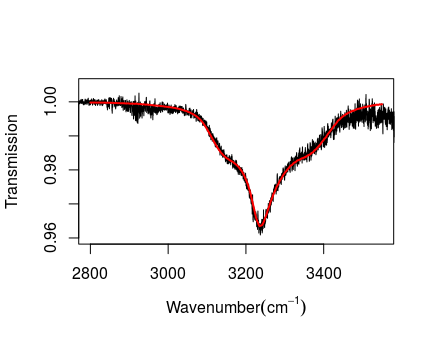
\includegraphics{figs/exSpec}
	\caption{An example spectrum from the ACE dataset, occultation ss48008, fit using the T-matrix code.}
	\label{fig:Fig1}
\end{figure}
occultation ss48008, at an altitude of 90.77 km. The raw spectrum has been smoothed to a resolution of 1 cm$^{-1}$. 
\begin{figure}
	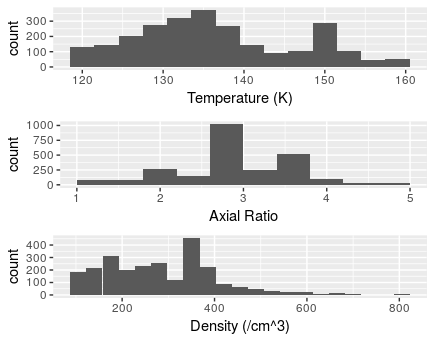
\includegraphics{figs/allHistograms}
	\caption{Distributions of temperature, particle shape (axial ratio) and density for all ACE spectra recorded from mission start to April 2017.}
	\label{fig:Fig2}
\end{figure}

\section{Results} \label{sec:results}
Figure \ref{fig:Fig2} shows the distribution of the three parameters of interest across all PMC detections. The cloud temperature and axial ratio, which appear to peak at $\approx$135 K and $\approx$2.9, respectively, agree reasonably well with the findings of AIM/SOFIE \cite{Hervig2010}. The bunch-up at $\approx$150 K in $T_{\text{ice}}$ could be attributed to the theoretical limit imposed by the frost point temperature, meaning that results beyond may not be believable. Finally, the volume density exhibits an exponential drop-off as is to be expected, and peaks at values near those found by MIPAS/Envisat \cite{Garcia-Comas2016}.  



\section{Discussion} \label{sec:disc}
In contrast with other instruments, ACE is able to measure PMCs year-round (with the exception of two, approximately two-week long periods in June and December when the satellite's geometry does not allow any measurements). Nevertheless, this ability has to this point never been exploited as a recurring data product. Even with this key advantage, it remains that PMC occurrences peak at the respective solstices in the Northern and Southern hemispheres. Thus, most of the opportunities for cross-comparison with other instruments result during this time. 
The Solar Occultation For Ice Experiment (SOFIE) was launched aboard the Aeronomy of Ice in the Mesosphere (AIM) satellite in 2007 at a 600 km polar orbit. It was designed with the sole goal of measuring PMCs and the surroundings in which they form. Like ACE, SOFIE uses solar occultations to derive extinction measures, but at 11 distinct wavelengths from 0.330 to 5.01 $\mu$m. 

\section{Conclusion} \label{sec:conc}


\section{References}
\bibliography{Bibliography}
\bibliographystyle{elsarticle-num}
\end{document}